\documentclass[pdftex12pt, a4paper]{article}
\usepackage[pdftex]{graphicx}
\usepackage{amsmath}
\usepackage{boxedminipage}
\usepackage{hyperref}
\usepackage{fullpage}

\begin{document}
\begin{titlepage}

\title{OSS Iteration 1}
\author{Michiel Huygen\\Tom Jacobs\\Victor Jacobs\\Jeroen Wygaerts}

\maketitle
\thispagestyle{empty}

\end{titlepage}

\newpage

\tableofcontents

\newpage


\section*{JSettlers}

The goal of the first part of this project for the course ``Ontwerp van softwaresystemen'' is to analyse an opensource-project, named JSettlers. 
This project is an implementation of the board game ``Settlers of Catan'' and is written in java.

\section{Introduction}
The analysis of the software was done on 2 parallel tracks. 
One track was to use code analysis tools to find problematic elements in the sourcecode. 
The other track used javadocs generated from the project's source. 
The javadoc gives a general idea of the distribution of responsiblities within the project.

The software seems to work without any problems; distributed setups cause no problems.

Our initial impression of the project is that very little time was spent on the actual software design. 
The documentation is extensive, although not 100\% complete. 
This seems necessary since the code is extremely incohesive. 
It seems an impressive feat that no bugs were encountered during our short tests of the software, considering the complexity of the code. 

\newpage
\section{Ontwerpdocumentatie}

\subsection{Domain model}
Settlers of Catan is originally a board game. 
The board consists of a number of hexagonal tiles which is depict a type of resource, ocean or desert. 
All resource tiles also have a Dice number on them. Several board pieces can be placed on the board. 
Cities and settlements are placed on the corner points of tiles. 
Roads and ships are placed on tile edges.
The robber is a piece that is place on the center of a tile
The game is turn based, each player plays his turn. 
A turn starts by rolling 2 dice. All cities and settlements next to a tile that has the rolled dice number on it recieve the resource depicted on the tile. Settlements give 1 resource per field, cities receive double.
Next the player can choose to spend resources by building TODOOOOO

\begin{figure}
\begin{center}
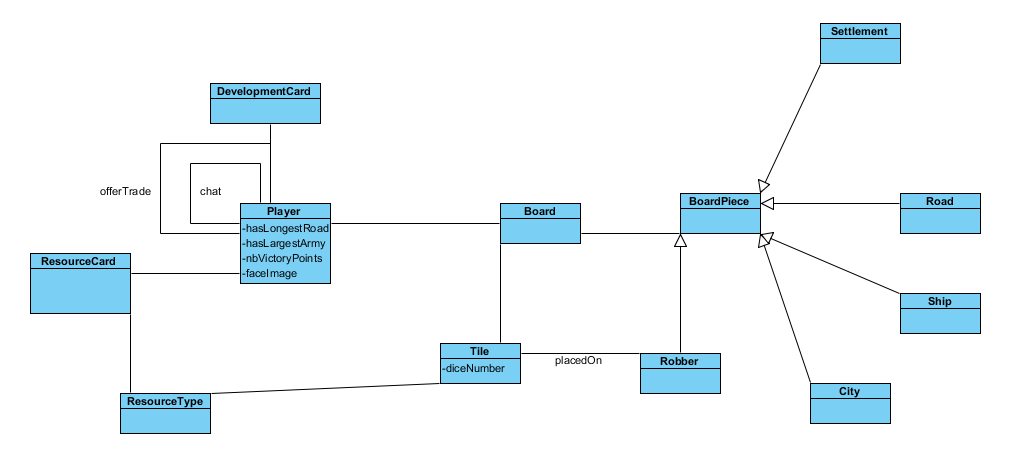
\includegraphics[width=1\textwidth]{Image/Ontwerp/DomainModel.png}
\caption{Domain model}
\label{fig:empty}
\end{center}
\end{figure}

\subsection{SOC.client package}
This package contains the code that makes up the Graphical User Interface.

The SOC.client package revolves around 3 God classes: SOCPlayerInterface, SOCHandPanel and SOCPlayerClient. 
They all contain dependencies to eachother. 
The remainder of the classes of this package can be divided into 2 parts. 
One part consists of helper classes used for user interface rendering. 
The other part contains mainly dialogs that are presented to the user and some panels that display a part of the game state. 
Almost all classes depend on one or more of the 3 god classes. 
In turn the 3 godclasses use all these parts to build the Client Interface.

\begin{figure}
\begin{center}
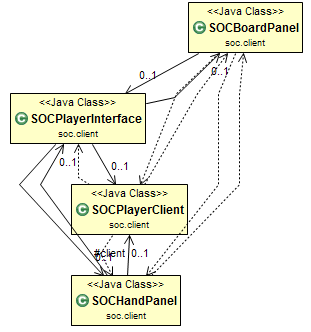
\includegraphics[width=0.4\textwidth]{Image/Ontwerp/ClientCore.png}
\caption{SOC.Client package overview}
\label{fig:empty}
\end{center}
\end{figure}

\subsection{SOC.game package}
This package holds the game state and data. 
A large part of this package contains a very complicated but seemingly ingenious way to work with the game board. 
(This is due to the board being hexagonal and board pieces being placed at corners or edges of tiles)

The main class in this package is the SOCGame class. 
It literally uses ALL other classes in this package. 
The class is used to store current game state and the game board, among other features.

\newpage

\section{Evaluatie ontwerp}

Maaanyy godclasses

The design structures that are present in the project seem to have been added while coding. 
There are some inheritance hierarchies present but it is not used for polymorfysm 

\section{Patronen}

\newpage

\section{Analysis}

Here some tools will be discussed that were used for analysing JSettlers code.
The first tool is Codecity, which displays the codebase. An other tool used was InCode, which delivers some interesting metrics about the code.
The last tool is CodePro

\subsection{Codecity}

Codecity really lives up to its name.
What it does is that it visualises the codebase by building a city out of it.
Buildings are classes with their dimensions directly correlated to the size of the class.
The height shows the number of methods in the class.
Width and length are both the number of attributes in the class.
Figure \ref{fig:codecityIso} shows an overview of the Codecity generated for JSettlers.

\begin{figure}
\begin{center}
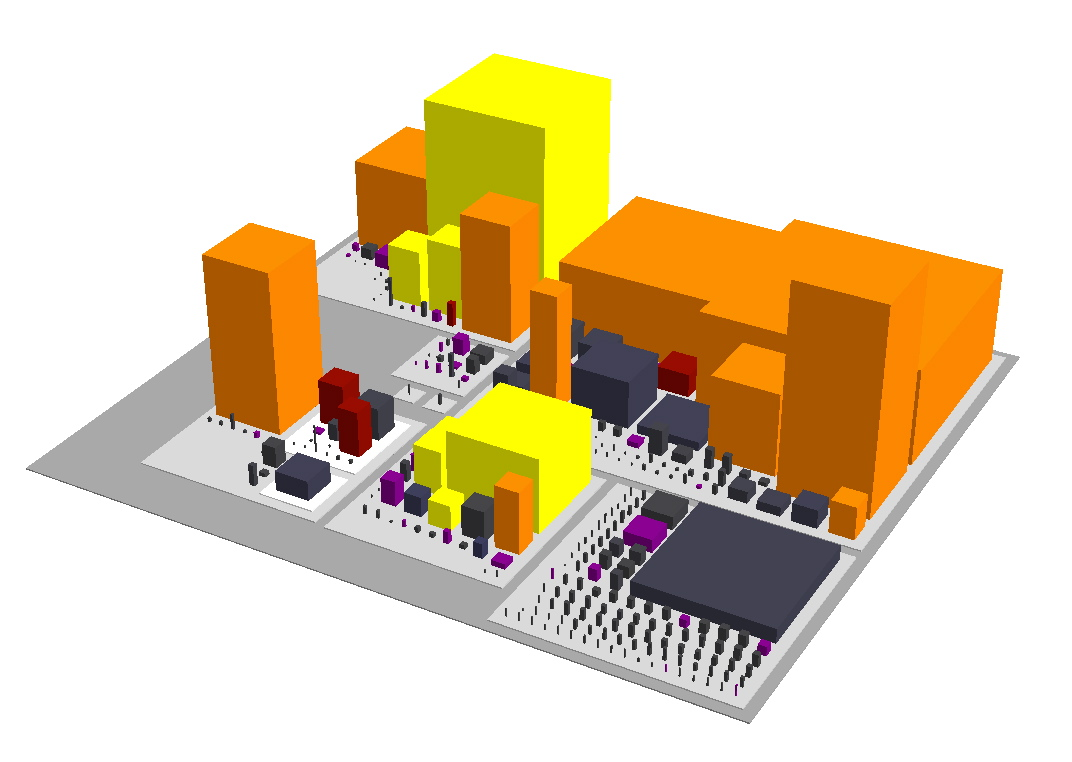
\includegraphics[width=0.8\textwidth]{Image/Codecity/Codecity2.jpg}
\caption{Isometric view of the JSettlers city}
\label{fig:codecityIso}
\end{center}
\end{figure}

The buildings in the figure are also color coded to easily spot the problems the individual classes have.
This is the so-called disharmony map.
The legend for the colors can be found in figure \ref{fig:legendCodeCity}.
There are numbers next to each type of problem, indicating how many classes are affected.

\begin{figure}
\begin{center}
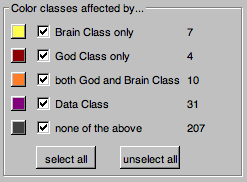
\includegraphics[width=0.4\textwidth]{Image/Codecity/Codecity4.png}
\caption{Color coding}
\label{fig:legendCodeCity}
\end{center}
\end{figure}

Codecity can distinguish between three types of problems:
\begin{description}
\item[God class] A God class is a class which \emph{knows too much or does too much}.
In other words, it's a class that does most of the work and delegates only minor things to other classes.
Therefore these classes tend to be very large and unwieldy.
This is very visible in figure \ref{fig:codecityIso}, where orange buildings are God classes.

The philosophy of OO programming is just the opposite to this centralisation: keep splitting up the project in smaller pieces until every individual fragment is of a manageable size.
It's also something that's very often found in OO projects, written by people who used to develop in a procedural language like C because they're used to write a program in one big file.

\item[Brain class] Brain classes 

\item[Data class] These are \emph{dumb} classes.
This means that they barely contain functionality and are mostly just for representing and storing data.

The problem with these classes is that they violate one of the basic ideas of OO programming, which is that an object represents a piece of data on which you can do operations.
Data classes obviously don't follow this idea because they only contain the data and no operations.

\end{description}

Another interesting view of the Codecity can be found in figure \ref{fig:codecityMap}.
Just as you might like to have a map of a city before you go exploring, Codecity can show a top-down view of the code.

\begin{figure}
\begin{center}
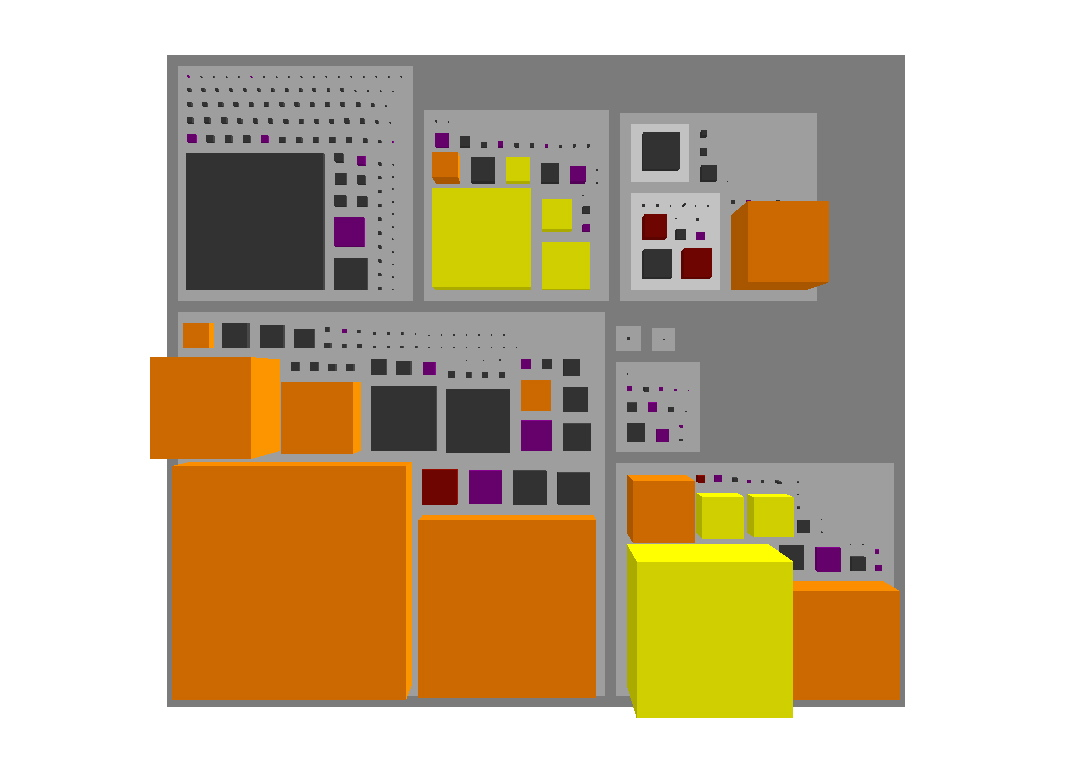
\includegraphics[width=0.8\textwidth]{Image/Codecity/Codecity3.jpg}
\caption{Map of the JSettlers city}
\label{fig:codecityMap}
\end{center}
\end{figure}

\subsection{inCode}

\begin{figure}
\begin{center}
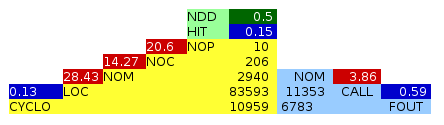
\includegraphics[width=0.6\textwidth]{Image/Incode/overview.png}
\caption{Overview from inCode}
\label{fig:incodeTriangle}
\end{center}
\end{figure}

\begin{figure}
\begin{center}
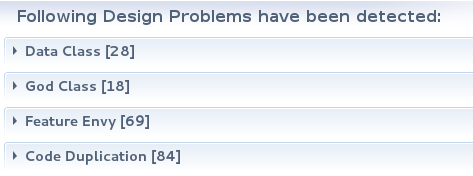
\includegraphics[width=0.6\textwidth]{Image/Incode/problems.png}
\caption{Problems found with inCode}
\label{fig:incodeTriangle}
\end{center}
\end{figure}

\subsection{CodePro}

CodePro is an entire suite of tools that goes from auditing code to code coverage, finding dead code and metrics.

\subsubsection{Audit}

JSettlers was audited with CodePro using the default rule set and the amount of bad programming practices in the codebase was staggering. Here are some of the things CodePro found:

\begin{itemize}
\item Catch clauses that catched \emph{Throwable}.
This is an easy hack if there's code that throws a number of exceptions and you don't want to write a specific case for every single one.
Although very easy this is generally not such a good idea since (at least in theory) every exception should be handled differently.
\item Instead of using \emph{.equals()} to check for equality between objects, \emph{==} was used an aweful lot.
This might be by design but it is very likely that someone was just not paying attention.
\item In some cases, variables were declared inside a loop instead of outside.
Declaring a variable in every iteration of the loop causes easily avoidable overhead.
\item Inconsistency in naming of variables, fields and even variables was a very frequent reoccurring problem.
\item Instead of doing something useful in a catch clause, many were just empty.
\end{itemize}

\subsubsection{Dead code}

CodePro found a \emph{lot} of dead code in the project.
Out of the 206 classes the project is made up of (see figure \ref{fig:incodeTriangle}, NOC), the tool insists that 67 are not used.
There's obviously something wrong with the tool for this test.

\subsubsection{Metrics}

The metrics are very similar to the pyramid found in figure \ref{fig:incodeTriangle} and will therefore not be repeated here.


\newpage

\section{Testen}

\newpage

\section{Besluit}

Hello 


\newpage

\section{Projectbeheer}

\end{document}